%
%
%

\label{sec:app_handlingpkm}

Further results for the case study of Section~\ref{sec:eval_handlingfreerotation} are given below.
Sketches of each possible resulting structure are shown in Figures	\ref{fig:handlingpkm_robots_3T0R_rev1}--\ref{fig:handlingpkm_robots_3T1R_pris} for redundant and prismatic actuation and for 3T0R and 3T1R motion.
%
The kinematic parameters are selected from the \propername{Pareto} diagrams in Figure~\ref{fig:handlingpkm_pareto} based on an equal weight for both criteria, normalized to the best-found value of each criterion.
The corresponding parameters are given in Tables~\ref{tab:handlingpkm_results_pris} and~\ref{tab:handlingpkm_results_pris_dh} for prismatic and Tables~\ref{tab:handlingpkm_results_rev} and~\ref{tab:handlingpkm_results_rev_dh} for revolute actuation.

\vspace{-6pt}
\begin{figure}[H] %
  \begin{adjustwidth}{-\extralength}{0cm}
    \centering
    \graphicspath{{Figures}}
    \input{./Figures/handlingpkm_robots_3T0R_rev.pdf_tex}
    \input{./Figures/handlingpkm_robots_3T0R_rev2.pdf_tex}
  \end{adjustwidth}
  \caption{Visualization %
    %
    of \emph{3T0R} parallel robots for the handling task with \emph{revolute} actuation. Markers are consistent with Figure~\ref{fig:handlingpkm_pareto}.}
  \label{fig:handlingpkm_robots_3T0R_rev1}
\end{figure}

%
%
  %
  %
  %
  %
%
%
%
\vspace{-6pt}
\begin{figure}[H]
  \begin{adjustwidth}{-\extralength}{0cm}
    \centering
    \graphicspath{{Figures}}
    \input{./Figures/handlingpkm_robots_3T1R_rev.pdf_tex}
  \end{adjustwidth}
  \caption[Handling task: Visualization of 3T1R parallel robots with revolute actuation]{Visualization of \emph{3T1R} parallel robots for the handling task with \emph{revolute} actuation.}
  \label{fig:handlingpkm_robots_3T1R_rev}
\end{figure}

\vspace{-6pt}
\begin{figure}[H]
  \begin{adjustwidth}{-\extralength}{0cm}
    \centering
    \graphicspath{{Figures}}
    \input{./Figures/handlingpkm_robots_3T0R_pris.pdf_tex}
  \end{adjustwidth}
  \caption[Handling task: Visualization of 3T0R parallel robots with prismatic actuation]{Visualization of \emph{3T0R} parallel robots for the handling task with \emph{prismatic} actuation. Markers are consistent with Figure~\ref{fig:handlingpkm_pareto}. Continued in Figure~\ref{fig:handlingpkm_robots_3T0R_pris2}.}
  \label{fig:handlingpkm_robots_3T0R_pris1}
\end{figure}

\vspace{-6pt}
\begin{figure}[H]
  \begin{adjustwidth}{-\extralength}{0cm}
    \centering
    \graphicspath{{Figures}}
    \input{./Figures/handlingpkm_robots_3T0R_pris2.pdf_tex}
  \end{adjustwidth}
  \caption[Handling task: Visualization of 3T0R parallel robots with prismatic actuation (p.~2)]{Visualization of \emph{3T0R} parallel robots (part~2), continuation of Figure~\ref{fig:handlingpkm_robots_3T0R_pris1}.}
  \label{fig:handlingpkm_robots_3T0R_pris2}
\end{figure}

\vspace{-6pt}
\begin{figure}[H]
  \begin{adjustwidth}{-\extralength}{0cm}
    \centering
    \graphicspath{{Figures}}
    \input{./Figures/handlingpkm_robots_3T1R_pris.pdf_tex}
  \end{adjustwidth}
  \caption[Handling task: Visualization of 3T1R parallel robots with prismatic actuation]{Visualization of \emph{3T1R} parallel robots for the handling task with \emph{prismatic} actuation.}
  \label{fig:handlingpkm_robots_3T1R_pris}
\end{figure}

\vspace{-10pt}

\begin{table}[H]
  \caption{Summary of the handling robot results (part 1, prismatic actuation)}
  \label{tab:handlingpkm_results_pris}
  \begin{adjustwidth}{-\extralength}{0cm}
    \centering
    \begin{tabularx}{\fulllength}{lRRRRRRRRRRRR} %
      \toprule
      \multicolumn{1}{c}{\textbf{Robot}}
      & \multicolumn{7}{c}{\textbf{Performance}} & \multicolumn{5}{c}{\textbf{Kinematic Parameters}} \\
      \midrule
      & \multicolumn{1}{r}{coll.} & \multicolumn{1}{r}{inst.spc.} & \multicolumn{1}{r}{footprt.}  & \multicolumn{1}{r}{power} & \multicolumn{1}{r}{force} & \multicolumn{1}{r}{velo.} & \multicolumn{1}{r}{cond.} &  \multicolumn{1}{c}{$n$} &
      \multicolumn{1}{c}{$r_\mathrm{b}$}  & \multicolumn{1}{c}{$\gamma_\mathrm{b}$} & \multicolumn{1}{c}{$r_\mathrm{p}$}  & \multicolumn{1}{c}{$\gamma_\mathrm{p}$} \\
      3T0R: & \multicolumn{1}{c}{mm} & \multicolumn{1}{c}{m$^3$} & \multicolumn{1}{c}{m$^2$} & \multicolumn{1}{c}{W} & \multicolumn{1}{c}{N} & \multicolumn{1}{c}{m/s} & \multicolumn{1}{c}{} & & \multicolumn{1}{c}{mm} &  \multicolumn{1}{c}{deg} & \multicolumn{1}{c}{mm} &  \multicolumn{1}{c}{deg}  \\
      \midrule %
      %
      \hyperrefl{restabrow:P3PRRR1GxPxA1}{3-\underline{\`P}{\`R}{\`R}{\`R}},\,c-m & 1 & 0.04 & 0.23 & 8.3 & 7.8 & 61 & 1.2 & 11 & 106 & 120 & 101 & 120 \\ % group 1; ARK_3T1R_20230728_plfabovejoints_rep1/Rob1_P3PRRR1G4P7A1 (Pareto-Index 2)
\midrule
\hyperrefl{restabrow:P3PRRRR3V1GxPxA1}{3-\underline{P}{R}{R}{U} var. 1},\,c-t & 0 & 0.08 & 0.29 & 11.5 & 9.4 & 70 & 1.4 & 11 & 100 & 63 & 100 & 0 \\ % group 3; ARK_3T1R_20230728_plfabovejoints2_rep2/Rob3_P3PRRRR3V1G4P2A1 (Pareto-Index 11)
\midrule
\hyperrefl{restabrow:P3PRRRR4GxPxA1}{3-\underline{\`P}{\`R}{\`R}{\'R}{\'R}},\,v-t & 0 & 0.08 & 0.21 & 34.1 & 13.4 & 146 & 6.0 & 12 & 207 & 0 & 100 & 0 \\ % group 4; ARK_3T1R_20230728_plfabovejoints2_rep2/Rob4_P3PRRRR4G1P2A1 (Pareto-Index 42)
\hyperrefl{restabrow:P3PRRRR4V1GxPxA1}{3-\underline{P}{R}{U}{R} var. 1},\,v-r & 0 & 0.11 & 0.21 & 26.6 & 8.7 & 176 & 7.2 & 10 & 110 & 0 & 100 & 0 \\ % group 5; ARK_3T1R_20230728_plfabovejoints2_rep2/Rob14_P3PRRRR4V1G1P3A1 (Pareto-Index 70)
\midrule
\hyperrefl{restabrow:P3PRRRR6GxPxA1}{3-\underline{P}{\`R}{\`R}{\'R}{\'R}},\,t-v & 4 & 0.07 & 0.27 & 17.8 & 10.2 & 100 & 4.6 & 11 & 156 & 0 & 100 & 0 \\ % group 6; ARK_3T1R_20230728_plfabovejoints2_rep2/Rob29_P3PRRRR6G2P1A1 (Pareto-Index 8)
\hyperrefl{restabrow:P3PRRRR6V1GxPxA1}{3-\underline{P}{R}{U}{R} var. 2},\,v-v & 3 & 0.07 & 0.19 & 14.8 & 6.7 & 126 & 6.3 & 10 & 122 & 0 & 121 & 0 \\ % group 7; ARK_3T1R_20230728_plfabovejoints2_rep2/Rob43_P3PRRRR6V1G1P1A1 (Pareto-Index 22)
\midrule
\hyperrefl{restabrow:P3PRRRR7GxPxA1}{3-\underline{P}{R}{\`R}{\`R}{\`R}},\,c-c & 26 & 0.07 & 0.44 & 6.4 & 5.1 & 72 & 1.4 & 13 & 100 & 95 & 101 & 45 \\ % group 9; ARK_3T1R_20230728_plfabovejoints2_rep1/Rob61_P3PRRRR7G4P9A1 (Pareto-Index 16)
\hyperrefl{restabrow:P3PRRRR7V1GxPxA1}{3-\underline{P}{U}{R}{R}},\,r-c & 5 & 0.06 & 0.39 & 8.2 & 6.0 & 78 & 1.0 & 10 & 100 & 0 & 101 & 36 \\ % group 10; ARK_3T1R_20230728_plfabovejoints_rep1/Rob63_P3PRRRR7V1G3P9A1 (Pareto-Index 3)
\midrule
\hyperrefl{restabrow:P3PRRRR8GxPxA1}{3-\underline{\`P}{\`R}{\'R}{\'R}{\`R}},\,r-t & 1 & 0.05 & 0.30 & 14.9 & 10.0 & 86 & 2.6 & 11 & 103 & 0 & 100 & 0 \\ % group 11; ARK_3T1R_20230728_plfabovejoints_rep2/Rob74_P3PRRRR8G3P2A1 (Pareto-Index 8)
\hyperrefl{restabrow:P3PRRRR8V1GxPxA1}{3-\underline{P}{U}{U}},\,t-r & 0 & 0.05 & 0.24 & 19.7 & 8.1 & 140 & 7.3 & 7 & 113 & 0 & 100 & 0 \\ % group 12; ARK_3T1R_20230728_plfabovejoints_rep1/Rob84_P3PRRRR8V1G2P3A1 (Pareto-Index 28)
\hyperrefl{restabrow:P3PRRRR8V2GxPxA1}{3-\underline{P}{R}{R}{U} var. 2},\,c-t & 4 & 0.06 & 0.23 & 12.7 & 7.7 & 94 & 3.6 & 10 & 100 & 73 & 100 & 0 \\ % group 13; ARK_3T1R_20230728_plfabovejoints2_rep1/Rob100_P3PRRRR8V2G4P2A1 (Pareto-Index 60)
\midrule
\hyperrefl{restabrow:P3RPRRR2V1GxPxA2}{3-{R}\underline{\`P}{\`R}{\`R}{\`R}},\,t-c & 42 & 0.08 & 0.31 & 5.3 & 6.4 & 47 & 2.0 & 11 & 108 & 0 & 100 & 55 \\ % group 15; ARK_3T1R_20230728_plfabovejoints2_rep1/Rob107_P3RPRRR2V1G2P9A1 (Pareto-Index 9)
\midrule
\hyperrefl{restabrow:P3RPRRR6V2GxPxA2}{3-{R}\underline{P}{R}{U} var. 1},\,v-v & 42 & 0.06 & 0.12 & 16.7 & 11.3 & 85 & 3.4 & 8 & 136 & 0 & 100 & 0 \\ % group 18; ARK_3T1R_20230728_plfabovejoints2_rep2/Rob108_P3RPRRR6V2G1P1A1 (Pareto-Index 75)
\hyperrefl{restabrow:P3RPRRR6V3GxPxA2}{3-{\`R}\underline{\`P}{\'R}{\'R}{\`R}},\,v-v & 28 & 0.09 & 0.15 & 23.6 & 13.6 & 99 & 5.6 & 10 & 236 & 0 & 100 & 0 \\ % group 19; ARK_3T1R_20230728_plfabovejoints_rep1/Rob111_P3RPRRR6V3G1P1A1 (Pareto-Index 3)
\midrule
\hyperrefl{restabrow:P3RPRRR8V2GxPxA2}{3-{R}\underline{P}{U}{R}},\,r-v & 49 & 0.05 & 0.24 & 12.8 & 10.5 & 70 & 3.9 & 7 & 100 & 0 & 100 & 0 \\ % group 20; ARK_3T1R_20230728_plfabovejoints2_rep1/Rob119_P3RPRRR8V2G3P1A1 (Pareto-Index 80)
\hyperrefl{restabrow:P3RPRRR8V3GxPxA2}{3-{\`R}\underline{P}{\`R}{\'R}{\'R}},\,r-v & 1 & 0.06 & 0.21 & 12.8 & 10.9 & 68 & 5.6 & 9 & 104 & 0 & 100 & 0 \\ % group 21; ARK_3T1R_20230728_plfabovejoints2_rep2/Rob129_P3RPRRR8V3G3P1A1 (Pareto-Index 241)
 \\
      \midrule
    \end{tabularx}
  \end{adjustwidth}
\end{table}



\begin{table}[H]\ContinuedFloat
  \caption[Handling task: Summary of the results (prismatic actuation)]{\emph{Cont.}}
%
  \begin{adjustwidth}{-\extralength}{0cm}
    \centering
    \begin{tabularx}{\fulllength}{lRRRRRRRRRRRR} %
      \toprule
      \multicolumn{1}{c}{\textbf{Robot}}
      & \multicolumn{7}{c}{\textbf{Performance}} & \multicolumn{5}{c}{\textbf{Kinematic Parameters}} \\
      \midrule
      \hyperrefl{restabrow:P3RPRRR9V2GxPxA2}{3-{R}\underline{P}{R}{U} var. 2},\,t-t & 8 & 0.06 & 0.16 & 11.5 & 10.7 & 62 & 3.3 & 8 & 330 & 0 & 111 & 0 \\ % group 22; ARK_3T1R_20230728_plfabovejoints2_rep1/Rob135_P3RPRRR9V2G2P2A1 (Pareto-Index 15)
\hyperrefl{restabrow:P3RPRRR9V3GxPxA2}{3-{\`R}\underline{\'P}{\'R}{\'R}{\`R}},\,t-t & 6 & 0.08 & 0.32 & 11.2 & 8.7 & 74 & 1.6 & 10 & 500 & 0 & 102 & 0 \\ % group 23; ARK_3T1R_20230728_plfabovejoints_rep1/Rob138_P3RPRRR9V3G2P2A1 (Pareto-Index 17)
\midrule
\hyperrefl{restabrow:P3RPRRR12V2GxPxA2}{3-{R}\underline{P}{R}{U} var. 3},\,t-t & 70 & 0.08 & 0.17 & 12.2 & 12.3 & 56 & 6.6 & 7 & 347 & 0 & 100 & 0 \\ % group 24; ARK_3T1R_20230728_plfabovejoints_rep1/Rob102_P3RPRRR12V2G2P2A1 (Pareto-Index 65)
\hyperrefl{restabrow:P3RPRRR12V3GxPxA2}{3-{\`R}\underline{P}{\'R}{\'R}{\`R}},\,r-r & 6 & 0.07 & 0.12 & 20.6 & 14.0 & 84 & 4.8 & 9 & 184 & 0 & 103 & 0 \\ % group 25; ARK_3T1R_20230728_plfabovejoints_rep1/Rob106_P3RPRRR12V3G3P3A1 (Pareto-Index 9)
\midrule
\hyperrefl{restabrow:P3RRPRR4V1GxPxA3}{3-{\`R}{\`R}\underline{\`P}{\'R}{\'R}},\,t-c & 6 & 0.06 & 0.46 & 22.4 & 12.1 & 106 & 3.4 & 11 & 127 & 0 & 102 & $-$60 \\ % group 26; ARK_3T1R_20230728_plfabovejoints2_rep1/Rob155_P3RRPRR4V1G2P9A1 (Pareto-Index 1)
\midrule
\hyperrefl{restabrow:P3RRPRR5V1GxPxA3}{3-{\`R}{\`R}\underline{\'P}{\'R}{\'R}},\,t-v & 0 & 0.07 & 0.14 & 25.6 & 12.6 & 117 & 4.5 & 10 & 224 & 0 & 110 & 0 \\ % group 29; ARK_3T1R_20230728_plfabovejoints2_rep2/Rob163_P3RRPRR5V1G2P1A1 (Pareto-Index 19)
\midrule
\hyperrefl{restabrow:P3RRPRR12V3GxPxA3}{3-{U}\underline{P}{U}},\,v-v & 11 & 0.03 & 0.12 & 10.8 & 9.4 & 66 & 2.8 & 5 & 127 & 0 & 102 & 0 \\ % group 30; ARK_3T1R_20230728_plfabovejoints_rep1/Rob140_P3RRPRR12V3G1P1A1 (Pareto-Index 213)
\hyperrefl{restabrow:P3RRPRR12V4GxPxA3}{3-{R}{R}\underline{P}{U}},\,v-v & 4 & 0.03 & 0.12 & 11.1 & 9.7 & 65 & 3.0 & 7 & 100 & 0 & 100 & 0 \\ % group 31; ARK_3T1R_20230728_plfabovejoints2_rep1/Rob143_P3RRPRR12V4G1P1A1 (Pareto-Index 79)
\hyperrefl{restabrow:P3RRPRR12V5GxPxA3}{3-{\`R}{\'R}\underline{P}{\'R}{\`R}},\,v-v & 1 & 0.04 & 0.12 & 10.3 & 8.9 & 66 & 2.5 & 9 & 172 & 0 & 100 & 0% group 32; ARK_3T1R_20230728_plfabovejoints2_rep1/Rob146_P3RRPRR12V5G1P1A1 (Pareto-Index 47) \\
      \midrule
      3T1R: & \multicolumn{7}{r}{} & \multicolumn{5}{r}{} \\
      \midrule
      \hyperrefl{restabrow:P4PRRRR6V1GxPxA1}{4-\underline{P}{R}{U}{R}},\,t-v & 6 & 0.19 & 0.73 & 16.1 & 12.1 & 77 & 4.4 & 9 & 327 & 0 & 282 & 0 \\ % group 8; ARK_3T1R_20230730_full_rep1/Rob220_P4PRRRR6V1G2P1A1 (Pareto-Index 4)
\midrule
\hyperrefl{restabrow:P4RPRRR8V2GxPxA2}{4-{R}\underline{P}{U}{R}},\,t-v & 32 & 0.20 & 0.44 & 17.3 & 12.3 & 80 & 31.2 & 7 & 223 & 0 & 171 & 0 \\ % group 16; ARK_3T1R_20230730_full_rep1/Rob231_P4RPRRR8V2G9P1A1 (Pareto-Index 3)
\hyperrefl{restabrow:P4RPRRR8V3GxPxA2}{4-{\`R}\underline{P}{\`R}{\'R}{\'R}},\,p-v & 1 & 0.18 & 0.42 & 15.3 & 10.2 & 86 & 28.5 & 9 & 202 & 0 & 169 & 0 \\ % group 17; ARK_3T1R_20230728_plfabovejoints2_rep1/Rob220_P4RPRRR8V3G9P1A1 (Pareto-Index 2)
\midrule
\hyperrefl{restabrow:P4RRPRR12V4GxPxA3}{4-{R}{R}\underline{P}{U}},\,v-v & 10 & 0.27 & 0.61 & 15.4 & 14.3 & 62 & 73.1 & 7 & 483 & 0 & 101 & 0 \\ % group 27; ARK_3T1R_20230729_v2_rep2/Rob24_P4RRPRR12V4G1P1A1 (Pareto-Index 1)
\hyperrefl{restabrow:P4RRPRR12V5GxPxA3}{4-{\`R}{\'R}\underline{P}{\'R}{\`R}},\,v-v & 7 & 0.23 & 0.51 & 12.7 & 13.3 & 55 & 36.5 & 9 & 384 & 0 & 216 & 0% group 28; ARK_3T1R_20230728_plfabovejoints_rep2/Rob222_P4RRPRR12V5G1P1A1 (Pareto-Index 8)
\\
      \midrule
      \cite{PrauseChaCor2015}: & \multicolumn{7}{l}{} & \multicolumn{5}{c}{From reference} \\ %
      \midrule
      3-\underline{C}RR & 54 & 0.08 & 0.33 & 10.4 & 8.8 & 68 & 1.2 & 11 & 300 & 120 & 110 & 120 \\ % Reference Solution; see eval_existing_design.m
\midrule
3-\underline{P}UU & 315 & 0.17 & 0.71 & 13.5 & 7.6 & 101 & 2.8 & 8 & 250 & $-$85 & 230 & 0 \\ % Reference Solution; see eval_existing_design.m
\midrule
3-\underline{C}RU & 4 & 0.17 & 0.54 & 0.7 & 8.3 & 5 & 8.0 & 10 & 300 & 115 & 420 & 0 \\ % Reference Solution; see eval_existing_design.m
\midrule
3-\underline{C}UR & 158 & 0.51 & 0.78 & 33.4 & 12.6 & 152 & 4.6 & 11 & 200 & 120 & 150 & 0 \\ % Reference Solution; see eval_existing_design.m
\midrule
3-U\underline{P}U & 150 & 0.12 & 0.32 & 8.8 & 8.1 & 63 & 2.1 & 5 & 500 & 0 & 120 & 0% Reference Solution; see eval_existing_design.m
\\
      \bottomrule
    \end{tabularx}
  \end{adjustwidth}
\end{table}

\vspace{-12pt}

\begin{table}[H]
  \centering
  \caption{Summary of the handling robot results (continuation of Table~\ref{tab:handlingpkm_results_pris}, leg-chain parameters).}
%
  \begin{adjustwidth}{-\extralength}{0cm}
    \centering %
    \begin{tabularx}{\fulllength}{lRRRRRRRRRRR} %
      \toprule
      \multicolumn{1}{c}{\textbf{Robot}}
      & \multicolumn{11}{c}{\textbf{Leg-Chain Kinematic Parameters}} \\
      \midrule
      & \multicolumn{1}{c}{$\alpha_{2}$} &		\multicolumn{1}{c}{$a_{2}$} & \multicolumn{1}{c}{$d_{2}$}
      & \multicolumn{1}{c}{$\alpha_{3}$} & \multicolumn{1}{c}{$a_{3}$} & \multicolumn{1}{c}{$d_{3}$} 
      & \multicolumn{1}{c}{$\alpha_{4}$} & \multicolumn{1}{c}{$a_{4}$} & \multicolumn{1}{c}{$d_{4}$} &
      \multicolumn{1}{c}{$a_{5}$} & \multicolumn{1}{c}{$d_{5}$}  \\						
      3T0R: & \multicolumn{1}{c}{deg} & \multicolumn{1}{c}{mm} & \multicolumn{1}{c}{mm} & \multicolumn{1}{c}{deg} & \multicolumn{1}{c}{mm} & \multicolumn{1}{c}{mm} & \multicolumn{1}{c}{deg} & \multicolumn{1}{c}{mm}& \multicolumn{1}{c}{mm} & \multicolumn{1}{c}{mm} & \multicolumn{1}{c}{mm}  \\
      \midrule %
      \hyperrefl{restabrow:P3PRRR1GxPxA1}{3-\underline{\`P}{\`R}{\`R}{\`R}},\,c-m & \textcolor{lightgray}{0} & \textcolor{lightgray}{0} & \textcolor{lightgray}{0} & \textcolor{lightgray}{0} & 183 & 154 & \textcolor{lightgray}{0} & 134 & 41 & \multicolumn{1}{c}{---} & \multicolumn{1}{c}{---} \\ % group 1; ARK_3T1R_20230728_plfabovejoints_rep1/Rob1_P3PRRR1G4P7A1 (Pareto-Index 2)
\midrule
\hyperrefl{restabrow:P3PRRRR3V1GxPxA1}{3-\underline{P}{R}{R}{U} var. 1},\,c-t & \textcolor{lightgray}{0} & \textcolor{lightgray}{0} & \textcolor{lightgray}{0} & \textcolor{lightgray}{0} & 131 & 25 & \textcolor{lightgray}{0} & 165 & 236 & \textcolor{lightgray}{0} & \textcolor{lightgray}{0} \\ % group 3; ARK_3T1R_20230728_plfabovejoints2_rep2/Rob3_P3PRRRR3V1G4P2A1 (Pareto-Index 11)
\midrule
\hyperrefl{restabrow:P3PRRRR4GxPxA1}{3-\underline{\`P}{\`R}{\`R}{\'R}{\'R}},\,v-t & \textcolor{lightgray}{0} & \textcolor{lightgray}{0} & \textcolor{lightgray}{0} & \textcolor{lightgray}{0} & 159 & 80 & \textcolor{lightgray}{90} & 149 & 3 & 274 & 1 \\ % group 4; ARK_3T1R_20230728_plfabovejoints2_rep2/Rob4_P3PRRRR4G1P2A1 (Pareto-Index 42)
\hyperrefl{restabrow:P3PRRRR4V1GxPxA1}{3-\underline{P}{R}{U}{R} var. 1},\,v-r & \textcolor{lightgray}{0} & \textcolor{lightgray}{0} & \textcolor{lightgray}{0} & \textcolor{lightgray}{0} & 284 & 33 & \textcolor{lightgray}{90} & \textcolor{lightgray}{0} & \textcolor{lightgray}{0} & 454 & 61 \\ % group 5; ARK_3T1R_20230728_plfabovejoints2_rep2/Rob14_P3PRRRR4V1G1P3A1 (Pareto-Index 70)
\midrule
\hyperrefl{restabrow:P3PRRRR6GxPxA1}{3-\underline{P}{\`R}{\`R}{\'R}{\'R}},\,t-v & \textcolor{lightgray}{90} & \textcolor{lightgray}{0} & \textcolor{lightgray}{0} & \textcolor{lightgray}{0} & 271 & 33 & \textcolor{lightgray}{90} & 151 & 30 & 227 & 27 \\ % group 6; ARK_3T1R_20230728_plfabovejoints2_rep2/Rob29_P3PRRRR6G2P1A1 (Pareto-Index 8)
\hyperrefl{restabrow:P3PRRRR6V1GxPxA1}{3-\underline{P}{R}{U}{R} var. 2},\,v-v & \textcolor{lightgray}{90} & \textcolor{lightgray}{0} & \textcolor{lightgray}{0} & \textcolor{lightgray}{0} & 493 & 0 & \textcolor{lightgray}{90} & \textcolor{lightgray}{0} & \textcolor{lightgray}{0} & 320 & 80 \\ % group 7; ARK_3T1R_20230728_plfabovejoints2_rep2/Rob43_P3PRRRR6V1G1P1A1 (Pareto-Index 22)
\midrule
\hyperrefl{restabrow:P3PRRRR7GxPxA1}{3-\underline{P}{R}{\`R}{\`R}{\`R}},\,c-c & \textcolor{lightgray}{90} & \textcolor{lightgray}{0} & \textcolor{lightgray}{0} & \textcolor{lightgray}{90} & 61 & 170 & \textcolor{lightgray}{0} & 148 & 174 & 165 & 57 \\ % group 9; ARK_3T1R_20230728_plfabovejoints2_rep1/Rob61_P3PRRRR7G4P9A1 (Pareto-Index 16)
\hyperrefl{restabrow:P3PRRRR7V1GxPxA1}{3-\underline{P}{U}{R}{R}},\,r-c & \textcolor{lightgray}{90} & \textcolor{lightgray}{0} & \textcolor{lightgray}{0} & \textcolor{lightgray}{90} & \textcolor{lightgray}{0} & \textcolor{lightgray}{0} & \textcolor{lightgray}{0} & 240 & 47 & 146 & 38 \\ % group 10; ARK_3T1R_20230728_plfabovejoints_rep1/Rob63_P3PRRRR7V1G3P9A1 (Pareto-Index 3)
\midrule
\hyperrefl{restabrow:P3PRRRR8GxPxA1}{3-\underline{\`P}{\`R}{\'R}{\'R}{\`R}},\,r-t & \textcolor{lightgray}{90} & \textcolor{lightgray}{0} & \textcolor{lightgray}{0} & \textcolor{lightgray}{90} & 25 & 42 & \textcolor{lightgray}{0} & 192 & 216 & 53 & 23 \\ % group 11; ARK_3T1R_20230728_plfabovejoints_rep2/Rob74_P3PRRRR8G3P2A1 (Pareto-Index 8)
\hyperrefl{restabrow:P3PRRRR8V1GxPxA1}{3-\underline{P}{U}{U}},\,t-r & \textcolor{lightgray}{90} & \textcolor{lightgray}{0} & \textcolor{lightgray}{0} & \textcolor{lightgray}{90} & \textcolor{lightgray}{0} & \textcolor{lightgray}{0} & \textcolor{lightgray}{0} & 299 & 135 & \textcolor{lightgray}{0} & \textcolor{lightgray}{0} \\ % group 12; ARK_3T1R_20230728_plfabovejoints_rep1/Rob84_P3PRRRR8V1G2P3A1 (Pareto-Index 28)
\hyperrefl{restabrow:P3PRRRR8V2GxPxA1}{3-\underline{P}{R}{R}{U} var. 2},\,c-t & \textcolor{lightgray}{90} & \textcolor{lightgray}{0} & \textcolor{lightgray}{0} & \textcolor{lightgray}{90} & 84 & 134 & \textcolor{lightgray}{0} & 153 & 128 & \textcolor{lightgray}{0} & \textcolor{lightgray}{0} \\ % group 13; ARK_3T1R_20230728_plfabovejoints2_rep1/Rob100_P3PRRRR8V2G4P2A1 (Pareto-Index 60)
\midrule
\hyperrefl{restabrow:P3RPRRR2V1GxPxA2}{3-{R}\underline{\`P}{\`R}{\`R}{\`R}},\,t-c & \textcolor{lightgray}{90} & \textcolor{lightgray}{0} & \textcolor{lightgray}{0} & \textcolor{lightgray}{0} & \textcolor{lightgray}{0} & \textcolor{lightgray}{0} & \textcolor{lightgray}{0} & 213 & 177 & 210 & 114 \\ % group 15; ARK_3T1R_20230728_plfabovejoints2_rep1/Rob107_P3RPRRR2V1G2P9A1 (Pareto-Index 9)
\midrule
\hyperrefl{restabrow:P3RPRRR6V2GxPxA2}{3-{R}\underline{P}{R}{U} var. 1},\,v-v & \textcolor{lightgray}{0} & \textcolor{lightgray}{0} & \textcolor{lightgray}{0} & \textcolor{lightgray}{90} & \textcolor{lightgray}{0} & \textcolor{lightgray}{0} & \textcolor{lightgray}{0} & 453 & 18 & \textcolor{lightgray}{0} & \textcolor{lightgray}{0} \\ % group 18; ARK_3T1R_20230728_plfabovejoints2_rep2/Rob108_P3RPRRR6V2G1P1A1 (Pareto-Index 75)
\hyperrefl{restabrow:P3RPRRR6V3GxPxA2}{3-{\`R}\underline{\`P}{\'R}{\'R}{\`R}},\,v-v & \textcolor{lightgray}{0} & \textcolor{lightgray}{0} & \textcolor{lightgray}{0} & \textcolor{lightgray}{90} & \textcolor{lightgray}{0} & \textcolor{lightgray}{0} & \textcolor{lightgray}{0} & 301 & 25 & 149 & 58 \\ % group 19; ARK_3T1R_20230728_plfabovejoints_rep1/Rob111_P3RPRRR6V3G1P1A1 (Pareto-Index 3)
\midrule
\hyperrefl{restabrow:P3RPRRR8V2GxPxA2}{3-{R}\underline{P}{U}{R}},\,r-v & \textcolor{lightgray}{90} & \textcolor{lightgray}{0} & \textcolor{lightgray}{0} & \textcolor{lightgray}{90} & \textcolor{lightgray}{0} & \textcolor{lightgray}{0} & \textcolor{lightgray}{90} & \textcolor{lightgray}{0} & \textcolor{lightgray}{0} & 281 & 2 \\ % group 20; ARK_3T1R_20230728_plfabovejoints2_rep1/Rob119_P3RPRRR8V2G3P1A1 (Pareto-Index 80)
\hyperrefl{restabrow:P3RPRRR8V3GxPxA2}{3-{\`R}\underline{P}{\`R}{\'R}{\'R}},\,r-v & \textcolor{lightgray}{90} & \textcolor{lightgray}{0} & \textcolor{lightgray}{0} & \textcolor{lightgray}{90} & \textcolor{lightgray}{0} & \textcolor{lightgray}{0} & \textcolor{lightgray}{90} & 3 & 44 & 274 & 4 \\ % group 21; ARK_3T1R_20230728_plfabovejoints2_rep2/Rob129_P3RPRRR8V3G3P1A1 (Pareto-Index 241)
 \\ %
      \midrule
    \end{tabularx}
  \end{adjustwidth}
\end{table}


\begin{table}[H]\ContinuedFloat
  \centering
  \caption{\emph{Cont.}} %
  \label{tab:handlingpkm_results_pris_dh}
  \begin{adjustwidth}{-\extralength}{0cm}
    \centering %
    \begin{tabularx}{\fulllength}{lRRRRRRRRRRR} %
      \toprule
      \multicolumn{1}{c}{\textbf{Robot}}
      & \multicolumn{11}{c}{\textbf{Leg-Chain Kinematic Parameters}} \\
      \midrule
      \hyperrefl{restabrow:P3RPRRR9V2GxPxA2}{3-{R}\underline{P}{R}{U} var. 2},\,t-t & \textcolor{lightgray}{90} & \textcolor{lightgray}{0} & \textcolor{lightgray}{0} & \textcolor{lightgray}{0} & \textcolor{lightgray}{0} & \textcolor{lightgray}{0} & \textcolor{lightgray}{0} & 157 & 83 & \textcolor{lightgray}{0} & \textcolor{lightgray}{0} \\ % group 22; ARK_3T1R_20230728_plfabovejoints2_rep1/Rob135_P3RPRRR9V2G2P2A1 (Pareto-Index 15)
\hyperrefl{restabrow:P3RPRRR9V3GxPxA2}{3-{\`R}\underline{\'P}{\'R}{\'R}{\`R}},\,t-t & \textcolor{lightgray}{90} & \textcolor{lightgray}{0} & \textcolor{lightgray}{0} & \textcolor{lightgray}{0} & \textcolor{lightgray}{0} & \textcolor{lightgray}{0} & \textcolor{lightgray}{0} & 161 & 45 & 3 & 0 \\ % group 23; ARK_3T1R_20230728_plfabovejoints_rep1/Rob138_P3RPRRR9V3G2P2A1 (Pareto-Index 17)
\midrule
\hyperrefl{restabrow:P3RPRRR12V2GxPxA2}{3-{R}\underline{P}{R}{U} var. 3},\,t-t & \textcolor{lightgray}{90} & \textcolor{lightgray}{0} & \textcolor{lightgray}{0} & \textcolor{lightgray}{90} & \textcolor{lightgray}{0} & \textcolor{lightgray}{0} & \textcolor{lightgray}{0} & 292 & 53 & \textcolor{lightgray}{0} & \textcolor{lightgray}{0} \\ % group 24; ARK_3T1R_20230728_plfabovejoints_rep1/Rob102_P3RPRRR12V2G2P2A1 (Pareto-Index 65)
\hyperrefl{restabrow:P3RPRRR12V3GxPxA2}{3-{\`R}\underline{P}{\'R}{\'R}{\`R}},\,r-r & \textcolor{lightgray}{90} & \textcolor{lightgray}{0} & \textcolor{lightgray}{0} & \textcolor{lightgray}{90} & \textcolor{lightgray}{0} & \textcolor{lightgray}{0} & \textcolor{lightgray}{0} & 391 & 6 & 21 & 73 \\ % group 25; ARK_3T1R_20230728_plfabovejoints_rep1/Rob106_P3RPRRR12V3G3P3A1 (Pareto-Index 9)
\midrule
\hyperrefl{restabrow:P3RRPRR4V1GxPxA3}{3-{\`R}{\`R}\underline{\`P}{\'R}{\'R}},\,t-c & \textcolor{lightgray}{0} & 201 & 275 & \textcolor{lightgray}{0} & \textcolor{lightgray}{0} & \textcolor{lightgray}{0} & \textcolor{lightgray}{90} & \textcolor{lightgray}{0} & \textcolor{lightgray}{0} & 299 & 63 \\ % group 26; ARK_3T1R_20230728_plfabovejoints2_rep1/Rob155_P3RRPRR4V1G2P9A1 (Pareto-Index 1)
\midrule
\hyperrefl{restabrow:P3RRPRR5V1GxPxA3}{3-{\`R}{\`R}\underline{\'P}{\'R}{\'R}},\,t-v & \textcolor{lightgray}{0} & 294 & 95 & \textcolor{lightgray}{90} & \textcolor{lightgray}{0} & \textcolor{lightgray}{0} & \textcolor{lightgray}{0} & \textcolor{lightgray}{0} & \textcolor{lightgray}{0} & 190 & 61 \\ % group 29; ARK_3T1R_20230728_plfabovejoints2_rep2/Rob163_P3RRPRR5V1G2P1A1 (Pareto-Index 19)
\midrule
\hyperrefl{restabrow:P3RRPRR12V3GxPxA3}{3-{U}\underline{P}{U}},\,v-v & \textcolor{lightgray}{90} & \textcolor{lightgray}{0} & \textcolor{lightgray}{0} & \textcolor{lightgray}{90} & \textcolor{lightgray}{0} & \textcolor{lightgray}{0} & \textcolor{lightgray}{90} & \textcolor{lightgray}{0} & \textcolor{lightgray}{0} & \textcolor{lightgray}{0} & \textcolor{lightgray}{0} \\ % group 30; ARK_3T1R_20230728_plfabovejoints_rep1/Rob140_P3RRPRR12V3G1P1A1 (Pareto-Index 213)
\hyperrefl{restabrow:P3RRPRR12V4GxPxA3}{3-{R}{R}\underline{P}{U}},\,v-v & \textcolor{lightgray}{90} & 22 & 35 & \textcolor{lightgray}{90} & \textcolor{lightgray}{0} & \textcolor{lightgray}{0} & \textcolor{lightgray}{90} & \textcolor{lightgray}{0} & \textcolor{lightgray}{0} & \textcolor{lightgray}{0} & \textcolor{lightgray}{0} \\ % group 31; ARK_3T1R_20230728_plfabovejoints2_rep1/Rob143_P3RRPRR12V4G1P1A1 (Pareto-Index 79)
\hyperrefl{restabrow:P3RRPRR12V5GxPxA3}{3-{\`R}{\'R}\underline{P}{\'R}{\`R}},\,v-v & \textcolor{lightgray}{90} & 21 & 37 & \textcolor{lightgray}{90} & \textcolor{lightgray}{0} & \textcolor{lightgray}{0} & \textcolor{lightgray}{90} & \textcolor{lightgray}{0} & \textcolor{lightgray}{0} & 20 & 8% group 32; ARK_3T1R_20230728_plfabovejoints2_rep1/Rob146_P3RRPRR12V5G1P1A1 (Pareto-Index 47)\\ %
      \midrule
      3T1R: & \multicolumn{11}{c}{} \\
      \midrule
      \hyperrefl{restabrow:P4PRRRR6V1GxPxA1}{4-\underline{P}{R}{U}{R}},\,t-v & \textcolor{lightgray}{90} & \textcolor{lightgray}{0} & \textcolor{lightgray}{0} & \textcolor{lightgray}{0} & 455 & 135 & \textcolor{lightgray}{90} & \textcolor{lightgray}{0} & \textcolor{lightgray}{0} & 419 & 74 \\ % group 8; ARK_3T1R_20230730_full_rep1/Rob220_P4PRRRR6V1G2P1A1 (Pareto-Index 4)
\midrule
\hyperrefl{restabrow:P4RPRRR8V2GxPxA2}{4-{R}\underline{P}{U}{R}},\,t-v & \textcolor{lightgray}{90} & \textcolor{lightgray}{0} & \textcolor{lightgray}{0} & \textcolor{lightgray}{90} & \textcolor{lightgray}{0} & \textcolor{lightgray}{0} & \textcolor{lightgray}{90} & \textcolor{lightgray}{0} & \textcolor{lightgray}{0} & 371 & 142 \\ % group 16; ARK_3T1R_20230730_full_rep1/Rob231_P4RPRRR8V2G9P1A1 (Pareto-Index 3)
\hyperrefl{restabrow:P4RPRRR8V3GxPxA2}{4-{\`R}\underline{P}{\`R}{\'R}{\'R}},\,p-v & \textcolor{lightgray}{90} & \textcolor{lightgray}{0} & \textcolor{lightgray}{0} & \textcolor{lightgray}{90} & \textcolor{lightgray}{0} & \textcolor{lightgray}{0} & \textcolor{lightgray}{90} & 35 & 30 & 292 & 126 \\ % group 17; ARK_3T1R_20230728_plfabovejoints2_rep1/Rob220_P4RPRRR8V3G9P1A1 (Pareto-Index 2)
\midrule
\hyperrefl{restabrow:P4RRPRR12V4GxPxA3}{4-{R}{R}\underline{P}{U}},\,v-v & \textcolor{lightgray}{90} & 153 & 155 & \textcolor{lightgray}{90} & \textcolor{lightgray}{0} & \textcolor{lightgray}{0} & \textcolor{lightgray}{90} & \textcolor{lightgray}{0} & \textcolor{lightgray}{0} & \textcolor{lightgray}{0} & \textcolor{lightgray}{0} \\ % group 27; ARK_3T1R_20230729_v2_rep2/Rob24_P4RRPRR12V4G1P1A1 (Pareto-Index 1)
\hyperrefl{restabrow:P4RRPRR12V5GxPxA3}{4-{\`R}{\'R}\underline{P}{\'R}{\`R}},\,v-v & \textcolor{lightgray}{90} & 191 & 8 & \textcolor{lightgray}{90} & \textcolor{lightgray}{0} & \textcolor{lightgray}{0} & \textcolor{lightgray}{90} & \textcolor{lightgray}{0} & \textcolor{lightgray}{0} & 90 & 16% group 28; ARK_3T1R_20230728_plfabovejoints_rep2/Rob222_P4RRPRR12V5G1P1A1 (Pareto-Index 8)
\\
      \midrule
      From \cite{PrauseChaCor2015}: & \multicolumn{11}{c}{Kinematic parameters from reference} \\
      \midrule
      3-\underline{C}RR & \textcolor{lightgray}{0} & \textcolor{lightgray}{0} & \textcolor{lightgray}{0} & \textcolor{lightgray}{0} & 290 & 0 & \textcolor{lightgray}{0} & 250 & 0 & \multicolumn{1}{c}{---} & \multicolumn{1}{c}{---} \\ % Reference Solution; see eval_existing_design.m
\midrule
3-\underline{P}UU & \textcolor{lightgray}{90} & \textcolor{lightgray}{0} & \textcolor{lightgray}{0} & \textcolor{lightgray}{90} & \textcolor{lightgray}{0} & \textcolor{lightgray}{0} & \textcolor{lightgray}{0} & 450 & 0 & \textcolor{lightgray}{0} & \textcolor{lightgray}{0} \\ % Reference Solution; see eval_existing_design.m
\midrule
3-\underline{C}RU & \textcolor{lightgray}{90} & \textcolor{lightgray}{0} & \textcolor{lightgray}{0} & \textcolor{lightgray}{90} & 100 & 0 & \textcolor{lightgray}{0} & 420 & 0 & \textcolor{lightgray}{0} & \textcolor{lightgray}{0} \\ % Reference Solution; see eval_existing_design.m
\midrule
3-\underline{C}UR & \textcolor{lightgray}{0} & \textcolor{lightgray}{0} & \textcolor{lightgray}{0} & \textcolor{lightgray}{0} & 490 & 0 & \textcolor{lightgray}{90} & \textcolor{lightgray}{0} & \textcolor{lightgray}{0} & 490 & 0 \\ % Reference Solution; see eval_existing_design.m
\midrule
3-U\underline{P}U & \textcolor{lightgray}{90} & \textcolor{lightgray}{0} & \textcolor{lightgray}{0} & \textcolor{lightgray}{90} & \textcolor{lightgray}{0} & \textcolor{lightgray}{0} & \textcolor{lightgray}{90} & \textcolor{lightgray}{0} & \textcolor{lightgray}{0} & \textcolor{lightgray}{0} & \textcolor{lightgray}{0}% Reference Solution; see eval_existing_design.m
\\
      \bottomrule
    \end{tabularx}
  \end{adjustwidth}
\end{table}


\vspace{-12pt}


\begin{table}[H]
  \tablesize{\fontsize{9}{9}\selectfont}
  \caption[Handling task: Summary of the results (revolute actuation)]{Summary of the handling robot results (part 2, revolute actuation).}
  \label{tab:handlingpkm_results_rev}
  \begin{adjustwidth}{-\extralength}{0cm}
    \begin{tabularx}{\fulllength}{lRRRRRRRRRRRR} %
      \toprule
      \multicolumn{1}{c}{\textbf{Robot}}
      & \multicolumn{7}{c}{\textbf{Performance}} & \multicolumn{5}{c}{\textbf{Kinematic Parameters}} \\
      \midrule
      & \multicolumn{1}{r}{coll.} & \multicolumn{1}{r}{inst.spc.} & \multicolumn{1}{r}{footprt.}  & \multicolumn{1}{r}{power} & \multicolumn{1}{r}{torque} & \multicolumn{1}{r}{velo.} & \multicolumn{1}{r}{cond.} &  \multicolumn{1}{c}{$n$} &
      \multicolumn{1}{c}{$r_\mathrm{b}$}  & \multicolumn{1}{c}{$\gamma_\mathrm{b}$} & \multicolumn{1}{c}{$r_\mathrm{p}$}  & \multicolumn{1}{c}{$\gamma_\mathrm{p}$} \\
      3T0R: & \multicolumn{1}{c}{mm} & \multicolumn{1}{c}{m$^3$} & \multicolumn{1}{c}{m$^2$} & \multicolumn{1}{c}{W} & \multicolumn{1}{c}{Nm} & \multicolumn{1}{c}{deg/s} & \multicolumn{1}{c}{} & & \multicolumn{1}{c}{mm} &  \multicolumn{1}{c}{deg} & \multicolumn{1}{c}{mm} &  \multicolumn{1}{c}{deg}  \\
      \midrule %
      %
      \hyperrefl{restabrow:P3RRRRR5GxPxA1}{3-\underline{\`R}{\`R}{\`R}{\'R}{\'R}},\,c-t & 3 & 0.07 & 0.16 & 41.1 & 1.7 & 455 & 3.3 & 14 & 122 & 100 & 103 & 0 \\ % group 40; ARK_3T1R_20230728_plfabovejoints_rep2/Rob187_P3RRRRR5G4P2A1 (Pareto-Index 6)
\hyperrefl{restabrow:P3RRRRR5V1GxPxA1}{3-\underline{R}{R}{U}{R} var. 1},\,r-t & 8 & 0.05 & 0.13 & 41.4 & 1.8 & 447 & 2.7 & 11 & 100 & 0 & 100 & 0 \\ % group 41; ARK_3T1R_20230730_full_rep1/Rob196_P3RRRRR5V1G3P2A1 (Pareto-Index 18)
\midrule
\hyperrefl{restabrow:P3RRRRR6GxPxA1}{3-\underline{\`R}{\`R}{\'R}{\'R}{\'R}},\,t-c & 3 & 0.08 & 0.34 & 24.6 & 1.1 & 436 & 3.1 & 14 & 344 & 0 & 100 & 60 \\ % group 42; ARK_3T1R_20230730_full_rep2/Rob200_P3RRRRR6G2P9A1 (Pareto-Index 26)
\hyperrefl{restabrow:P3RRRRR6V1GxPxA1}{3-\underline{R}{U}{R}{R}},\,t-c & 16 & 0.06 & 0.30 & 23.2 & 1.0 & 430 & 2.6 & 12 & 299 & 0 & 100 & 55 \\ % group 43; ARK_3T1R_20230730_full_rep2/Rob201_P3RRRRR6V1G2P9A1 (Pareto-Index 54)
\midrule
\hyperrefl{restabrow:P3RRRRR7GxPxA1}{3-\underline{\`R}{\'R}{\'R}{\'R}{\`R}},\,t-t & 17 & 0.05 & 0.16 & 57.7 & 2.5 & 439 & 4.1 & 13 & 119 & 0 & 100 & 0 \\ % group 44; ARK_3T1R_20230730_full_rep1/Rob202_P3RRRRR7G2P2A1 (Pareto-Index 25)
\hyperrefl{restabrow:P3RRRRR7V2GxPxA1}{3-\underline{R}{R}{R}{U} var. 1},\,t-t & 2 & 0.04 & 0.14 & 56.9 & 2.5 & 433 & 4.2 & 11 & 117 & 0 & 100 & 0 \\ % group 45; ARK_3T1R_20230730_v1_rep2/Rob204_P3RRRRR7V2G2P2A1 (Pareto-Index 10)
\midrule
\hyperrefl{restabrow:P3RRRRR8GxPxA1}{3-\underline{\`R}{\'R}{\'R}{\`R}{\`R}},\,r-r & 0 & 0.05 & 0.18 & 43.9 & 1.8 & 454 & 3.8 & 13 & 104 & 0 & 100 & 0 \\ % group 46; ARK_3T1R_20230730_v1_rep3/Rob208_P3RRRRR8G3P3A1 (Pareto-Index 2)
\hyperrefl{restabrow:P3RRRRR8V2GxPxA1}{3-\underline{R}{R}{U}{R} var. 2},\,r-r & 7 & 0.04 & 0.17 & 45.6 & 2.0 & 439 & 4.2 & 11 & 100 & 0 & 100 & 0 \\ % group 47; ARK_3T1R_20230728_plfabovejoints_rep1/Rob211_P3RRRRR8V2G3P3A1 (Pareto-Index 10)
\midrule
\hyperrefl{restabrow:P3RRRRR10GxPxA1}{3-\underline{\`R}{\`R}{\'R}{\'R}{\`R}},\,r-r & 18 & 0.04 & 0.15 & 40.7 & 1.7 & 456 & 3.7 & 13 & 126 & 0 & 103 & 0 \\ % group 48; ARK_3T1R_20230728_plfabovejoints_rep2/Rob173_P3RRRRR10G3P3A1 (Pareto-Index 4)
\hyperrefl{restabrow:P3RRRRR10V1GxPxA1}{3-\underline{R}{U}{U}},\,r-r & 57 & 0.04 & 0.13 & 45.1 & 1.9 & 452 & 4.2 & 9 & 107 & 0 & 100 & 0 \\ % group 49; ARK_3T1R_20230730_v1_rep2/Rob176_P3RRRRR10V1G3P3A1 (Pareto-Index 140)
\hyperrefl{restabrow:P3RRRRR10V2GxPxA1}{3-\underline{R}{R}{R}{U} var. 2},\,r-r & 12 & 0.04 & 0.13 & 40.0 & 1.7 & 450 & 3.1 & 11 & 152 & 0 & 104 & 0% group 50; ARK_3T1R_20230730_v1_rep2/Rob179_P3RRRRR10V2G3P3A1 (Pareto-Index 7)
\\ %
      \midrule
      3T1R: & \multicolumn{7}{r}{} & \multicolumn{5}{r}{} \\
      \midrule
      \hyperrefl{restabrow:P4RRRRR5GxPxA1}{4-\underline{\`R}{\`R}{\`R}{\'R}{\'R}},\,r-v & 18 & 0.13 & 0.42 & 15.8 & 2.0 & 451 & 38.1 & 13 & 270 & 0 & 203 & 0 \\ % group 33; ARK_3T1R_20230730_full_rep2/Rob253_P4RRRRR5G3P1A1 (Pareto-Index 3)
\hyperrefl{restabrow:P4RRRRR5V1GxPxA1}{4-\underline{R}{R}{U}{R} var. 1},\,t-v & 0 & 0.11 & 0.46 & 74.5 & 2.4 & 453 & 90.3 & 11 & 349 & 0 & 109 & 0 \\ % group 34; ARK_3T1R_20230730_full_rep1/Rob257_P4RRRRR5V1G2P1A1 (Pareto-Index 17)
\midrule
\hyperrefl{restabrow:P4RRRRR8GxPxA1}{4-\underline{\`R}{\'R}{\'R}{\`R}{\`R}},\,v-v & 0 & 0.19 & 0.59 & 125.5 & 4.2 & 428 & 19.8 & 13 & 372 & 0 & 100 & 0 \\ % group 35; ARK_3T1R_20230730_full_rep1/Rob260_P4RRRRR8G1P1A1 (Pareto-Index 7)
\hyperrefl{restabrow:P4RRRRR8V2GxPxA1}{4-\underline{R}{R}{U}{R} var. 2},\,v-v & 0 & 0.16 & 0.83 & 375.8 & 14.0 & 384 & 30.7 & 11 & 403 & 0 & 122 & 0 \\ % group 36; ARK_3T1R_20230730_full_rep2/Rob261_P4RRRRR8V2G1P1A1 (Pareto-Index 2)
\midrule
\hyperrefl{restabrow:P4RRRRR10GxPxA1}{4-\underline{\`R}{\`R}{\'R}{\'R}{\`R}},\,v-v & 11 & 0.10 & 0.74 & 322.9 & 10.7 & 433 & 49.6 & 13 & 491 & 0 & 102 & 0 \\ % group 37; ARK_3T1R_20230730_full_rep2/Rob246_P4RRRRR10G1P1A1 (Pareto-Index 2)
\hyperrefl{restabrow:P4RRRRR10V1GxPxA1}{4-\underline{R}{U}{U}},\,v-v & 15 & 0.14 & 0.69 & 110.6 & 3.6 & 436 & 27.9 & 9 & 453 & 0 & 126 & 0 \\ % group 38; ARK_3T1R_20230730_full_rep2/Rob247_P4RRRRR10V1G1P1A1 (Pareto-Index 12)
\hyperrefl{restabrow:P4RRRRR10V2GxPxA1}{4-\underline{R}{R}{R}{U}},\,v-v & 7 & 0.12 & 0.62 & 400.4 & 12.7 & 451 & 46.7 & 11 & 468 & 0 & 147 & 0% group 39; ARK_3T1R_20230730_full_rep2/Rob248_P4RRRRR10V2G1P1A1 (Pareto-Index 2)
\\ %
      \bottomrule
    \end{tabularx}
  \end{adjustwidth}
\end{table}

\begin{table}[H]
  \caption[Handling task: Summary of the results (leg chain kinematic parameters, revolute actuation)]{\textls[-15]{Summary of the handling robot results (part 2 continuation of Table~\ref{tab:handlingpkm_results_rev}, leg chain parameters).}}
  \label{tab:handlingpkm_results_rev_dh}
  \begin{adjustwidth}{-\extralength}{0cm}
    \centering
    \begin{tabularx}{\fulllength}{lRRRRRRRRRRR} %
      \toprule
      \multicolumn{1}{c}{\textbf{Robot}}
      & \multicolumn{11}{c}{\textbf{Leg-chain kinematic parameters}} \\
      \midrule
      & \multicolumn{1}{c}{$\alpha_{2}$} &		\multicolumn{1}{c}{$a_{2}$} & \multicolumn{1}{c}{$d_{2}$}
      & \multicolumn{1}{c}{$\alpha_{3}$} & \multicolumn{1}{c}{$a_{3}$} & \multicolumn{1}{c}{$d_{3}$} 
      & \multicolumn{1}{c}{$\alpha_{4}$} & \multicolumn{1}{c}{$a_{4}$} & \multicolumn{1}{c}{$d_{4}$} &
      \multicolumn{1}{c}{$a_{5}$} & \multicolumn{1}{c}{$d_{5}$}  \\						
      3T0R: & \multicolumn{1}{c}{deg} & \multicolumn{1}{c}{mm} & \multicolumn{1}{c}{mm} & \multicolumn{1}{c}{deg} & \multicolumn{1}{c}{mm} & \multicolumn{1}{c}{mm} & \multicolumn{1}{c}{deg} & \multicolumn{1}{c}{mm}& \multicolumn{1}{c}{mm} & \multicolumn{1}{c}{mm} & \multicolumn{1}{c}{mm}  \\
      \midrule %
      \hyperrefl{restabrow:P3RRRRR5GxPxA1}{3-\underline{\`R}{\`R}{\`R}{\'R}{\'R}},\,c-t & \textcolor{lightgray}{0} & 184 & 44 & \textcolor{lightgray}{0} & 174 & 13 & \textcolor{lightgray}{90} & 17 & 48 & 276 & 66 \\ % group 40; ARK_3T1R_20230728_plfabovejoints_rep2/Rob187_P3RRRRR5G4P2A1 (Pareto-Index 6)
\hyperrefl{restabrow:P3RRRRR5V1GxPxA1}{3-\underline{R}{R}{U}{R} var. 1},\,r-t & \textcolor{lightgray}{0} & 197 & 44 & \textcolor{lightgray}{0} & 225 & 45 & \textcolor{lightgray}{90} & \textcolor{lightgray}{0} & \textcolor{lightgray}{0} & 204 & 47 \\ % group 41; ARK_3T1R_20230730_full_rep1/Rob196_P3RRRRR5V1G3P2A1 (Pareto-Index 18)
\midrule
\hyperrefl{restabrow:P3RRRRR6GxPxA1}{3-\underline{\`R}{\`R}{\'R}{\'R}{\'R}},\,t-c & \textcolor{lightgray}{0} & 166 & 165 & \textcolor{lightgray}{90} & 20 & 117 & \textcolor{lightgray}{0} & 206 & 89 & 196 & 16 \\ % group 42; ARK_3T1R_20230730_full_rep2/Rob200_P3RRRRR6G2P9A1 (Pareto-Index 26)
\hyperrefl{restabrow:P3RRRRR6V1GxPxA1}{3-\underline{R}{U}{R}{R}},\,t-c & \textcolor{lightgray}{0} & 161 & 161 & \textcolor{lightgray}{90} & \textcolor{lightgray}{0} & \textcolor{lightgray}{0} & \textcolor{lightgray}{0} & 196 & 73 & 177 & 37 \\ % group 43; ARK_3T1R_20230730_full_rep2/Rob201_P3RRRRR6V1G2P9A1 (Pareto-Index 54)
\midrule
\hyperrefl{restabrow:P3RRRRR7GxPxA1}{3-\underline{\`R}{\'R}{\'R}{\'R}{\`R}},\,t-t & \textcolor{lightgray}{90} & 3 & 74 & \textcolor{lightgray}{0} & 175 & 30 & \textcolor{lightgray}{0} & 169 & 157 & 14 & 19 \\ % group 44; ARK_3T1R_20230730_full_rep1/Rob202_P3RRRRR7G2P2A1 (Pareto-Index 25)
\hyperrefl{restabrow:P3RRRRR7V2GxPxA1}{3-\underline{R}{R}{R}{U} var. 1},\,t-t & \textcolor{lightgray}{90} & 36 & 26 & \textcolor{lightgray}{0} & 161 & 21 & \textcolor{lightgray}{0} & 146 & 161 & \textcolor{lightgray}{0} & \textcolor{lightgray}{0} \\ % group 45; ARK_3T1R_20230730_v1_rep2/Rob204_P3RRRRR7V2G2P2A1 (Pareto-Index 10)
\midrule
\hyperrefl{restabrow:P3RRRRR8GxPxA1}{3-\underline{\`R}{\'R}{\'R}{\`R}{\`R}},\,r-r & \textcolor{lightgray}{90} & 164 & 48 & \textcolor{lightgray}{0} & 196 & 52 & \textcolor{lightgray}{90} & 175 & 41 & 180 & 31 \\ % group 46; ARK_3T1R_20230730_v1_rep3/Rob208_P3RRRRR8G3P3A1 (Pareto-Index 2)
\hyperrefl{restabrow:P3RRRRR8V2GxPxA1}{3-\underline{R}{R}{U}{R} var. 2},\,r-r & \textcolor{lightgray}{90} & 1 & 72 & \textcolor{lightgray}{0} & 212 & 39 & \textcolor{lightgray}{90} & \textcolor{lightgray}{0} & \textcolor{lightgray}{0} & 176 & 4 \\ % group 47; ARK_3T1R_20230728_plfabovejoints_rep1/Rob211_P3RRRRR8V2G3P3A1 (Pareto-Index 10)
\midrule
\hyperrefl{restabrow:P3RRRRR10GxPxA1}{3-\underline{\`R}{\`R}{\'R}{\'R}{\`R}},\,r-r & \textcolor{lightgray}{0} & 175 & 25 & \textcolor{lightgray}{90} & 22 & 63 & \textcolor{lightgray}{0} & 181 & 108 & 5 & 7 \\ % group 48; ARK_3T1R_20230728_plfabovejoints_rep2/Rob173_P3RRRRR10G3P3A1 (Pareto-Index 4)
\hyperrefl{restabrow:P3RRRRR10V1GxPxA1}{3-\underline{R}{U}{U}},\,r-r & \textcolor{lightgray}{0} & 173 & 0 & \textcolor{lightgray}{90} & \textcolor{lightgray}{0} & \textcolor{lightgray}{0} & \textcolor{lightgray}{0} & 235 & 126 & \textcolor{lightgray}{0} & \textcolor{lightgray}{0} \\ % group 49; ARK_3T1R_20230730_v1_rep2/Rob176_P3RRRRR10V1G3P3A1 (Pareto-Index 140)
\hyperrefl{restabrow:P3RRRRR10V2GxPxA1}{3-\underline{R}{R}{R}{U} var. 2},\,r-r & \textcolor{lightgray}{0} & 175 & 53 & \textcolor{lightgray}{90} & 50 & 158 & \textcolor{lightgray}{0} & 170 & 35 & \textcolor{lightgray}{0} & \textcolor{lightgray}{0}% group 50; ARK_3T1R_20230730_v1_rep2/Rob179_P3RRRRR10V2G3P3A1 (Pareto-Index 7)
\\
      \midrule
      3T1R: & \multicolumn{11}{c}{} \\
      \midrule
      \hyperrefl{restabrow:P4RRRRR5GxPxA1}{4-\underline{\`R}{\`R}{\`R}{\'R}{\'R}},\,r-v & \textcolor{lightgray}{0} & 213 & 53 & \textcolor{lightgray}{0} & 167 & 100 & \textcolor{lightgray}{90} & 217 & 51 & 225 & 2 \\ % group 33; ARK_3T1R_20230730_full_rep2/Rob253_P4RRRRR5G3P1A1 (Pareto-Index 3)
\hyperrefl{restabrow:P4RRRRR5V1GxPxA1}{4-\underline{R}{R}{U}{R} var. 1},\,t-v & \textcolor{lightgray}{0} & 199 & 73 & \textcolor{lightgray}{0} & 178 & 52 & \textcolor{lightgray}{90} & \textcolor{lightgray}{0} & \textcolor{lightgray}{0} & 219 & 2 \\ % group 34; ARK_3T1R_20230730_full_rep1/Rob257_P4RRRRR5V1G2P1A1 (Pareto-Index 17)
\midrule
\hyperrefl{restabrow:P4RRRRR8GxPxA1}{4-\underline{\`R}{\'R}{\'R}{\`R}{\`R}},\,v-v & \textcolor{lightgray}{90} & 91 & 113 & \textcolor{lightgray}{0} & 290 & 164 & \textcolor{lightgray}{90} & 59 & 80 & 274 & 125 \\ % group 35; ARK_3T1R_20230730_full_rep1/Rob260_P4RRRRR8G1P1A1 (Pareto-Index 7)
\hyperrefl{restabrow:P4RRRRR8V2GxPxA1}{4-\underline{R}{R}{U}{R} var. 2},\,v-v & \textcolor{lightgray}{90} & 20 & 335 & \textcolor{lightgray}{0} & 204 & 18 & \textcolor{lightgray}{90} & \textcolor{lightgray}{0} & \textcolor{lightgray}{0} & 336 & 80 \\ % group 36; ARK_3T1R_20230730_full_rep2/Rob261_P4RRRRR8V2G1P1A1 (Pareto-Index 2)
\midrule
\hyperrefl{restabrow:P4RRRRR10GxPxA1}{4-\underline{\`R}{\`R}{\'R}{\'R}{\`R}},\,v-v & \textcolor{lightgray}{0} & 257 & 41 & \textcolor{lightgray}{90} & 172 & 64 & \textcolor{lightgray}{0} & 250 & 30 & 21 & 5 \\ % group 37; ARK_3T1R_20230730_full_rep2/Rob246_P4RRRRR10G1P1A1 (Pareto-Index 2)
\hyperrefl{restabrow:P4RRRRR10V1GxPxA1}{4-\underline{R}{U}{U}},\,v-v & \textcolor{lightgray}{0} & 274 & 45 & \textcolor{lightgray}{90} & \textcolor{lightgray}{0} & \textcolor{lightgray}{0} & \textcolor{lightgray}{0} & 384 & 131 & \textcolor{lightgray}{0} & \textcolor{lightgray}{0} \\ % group 38; ARK_3T1R_20230730_full_rep2/Rob247_P4RRRRR10V1G1P1A1 (Pareto-Index 12)
\hyperrefl{restabrow:P4RRRRR10V2GxPxA1}{4-\underline{R}{R}{R}{U}},\,v-v & \textcolor{lightgray}{0} & 265 & 74 & \textcolor{lightgray}{90} & 69 & 167 & \textcolor{lightgray}{0} & 237 & 47 & \textcolor{lightgray}{0} & \textcolor{lightgray}{0}% group 39; ARK_3T1R_20230730_full_rep2/Rob248_P4RRRRR10V2G1P1A1 (Pareto-Index 2)
\\
      \bottomrule
    \end{tabularx}
  \end{adjustwidth}
\end{table}


%

The \propername{Pareto} diagram in Figure~\ref{fig:handlingpkm_pareto_prismatic_onlypoints} 
%
corresponds to the one in Figure~\ref{fig:handlingpkm_pareto}a.
It is based on the optimization only using the 27 reference points, not the reference trajectory with \mbox{4851 samples}.
Thereby, the results are based on the same assumptions as the study in \cite{PrauseChaCor2015}.

%
%
%
%
%

For a direct comparison with \cite{PrauseChaCor2015}, sketches of the optimal results from the paper are given in Figure~\ref{fig:handlingpkm_robots_reference}.
Especially for 3-\underline{P}UU (Figure \ref{fig:handlingpkm_robots_reference}b), 3-\underline{C}RU (Figure \ref{fig:handlingpkm_robots_reference}c), and 3-\underline{C}UR (Figure \ref{fig:handlingpkm_robots_reference}d), large structures have been found by \cite{PrauseChaCor2015} that are outperformed by the results of this replication of the study.
%
The box plots from the paper (Figure~\ref{fig:handlingpkm_boxplot_PrauseChaCor2015}b,d,e) are compared to the reproduction by the proposed synthesis toolchain (in Figure~\ref{fig:handlingpkm_boxplot_PrauseChaCor2015}a,c,e) for different criteria, as explained in Section~\ref{sec:eval_handling_results}.

%
The following pages give different performance maps for the resolution of the functional redundancy of the 3T1R parallel robots within the handling task.
Each page contains the maps of all robots for one heat-map criterion.
The always identical trajectory comes from the dimensional synthesis, where the minimization of actuator force or torque was selected as the IK objective. %
The robots with prismatic actuation are given at the top \mbox{(Figures~\ref{fig:handlingpkm_perfmaps_multi_actforce_pris}, ~\ref{fig:handlingpkm_perfmaps_multi_poserr_pris}}, and~\ref{fig:handlingpkm_perfmaps_multi_condikjac_pris}), and with revolute actuation at the bottom of the pages \mbox{(Figures~\ref{fig:handlingpkm_perfmaps_multi_actforce_rev}, ~\ref{fig:handlingpkm_perfmaps_multi_poserr_rev}, and~\ref{fig:handlingpkm_perfmaps_multi_condikjac_rev})}.
The actuator-force/torque maps (Figures~\ref{fig:handlingpkm_perfmaps_multi_actforce_pris} and~\ref{fig:handlingpkm_perfmaps_multi_actforce_rev}) show the ability of the redundancy resolution to minimize the actuator forces by avoiding areas of high required force (dark colors). %
For most structures, however, the force necessary in the reachable orientations is relatively uniform.
The limitation of the end-effector precision to \SI{500}{\micro\metre} %
is only influencing the 3T1R PRs with prismatic actuation, as is visible in Figure~\ref{fig:handlingpkm_perfmaps_multi_poserr_pris}.
The error is much lower for revolute actuation in Figure~\ref{fig:handlingpkm_perfmaps_multi_poserr_rev}. %
Since the position error is proportional to the assumed encoder accuracy, principally better precision of the revolute actuation cannot be concluded, as a strictly equivalent selection of encoders was not subject to the case study. %
The heat maps in Figures~\ref{fig:handlingpkm_perfmaps_multi_condikjac_pris} and~\ref{fig:handlingpkm_perfmaps_multi_condikjac_rev} show the condition number of the full inverse-kinematics matrix (``IK \propername{Jacobian}'', see \cite{SchapplerTapOrt2019c}, connected to the IK singularities within the workspace of 3T1R PRs, especially with revolute actuation. %
%
%

\begin{figure}[H]
  \begin{adjustwidth}{-\extralength}{0cm}
    \centering
    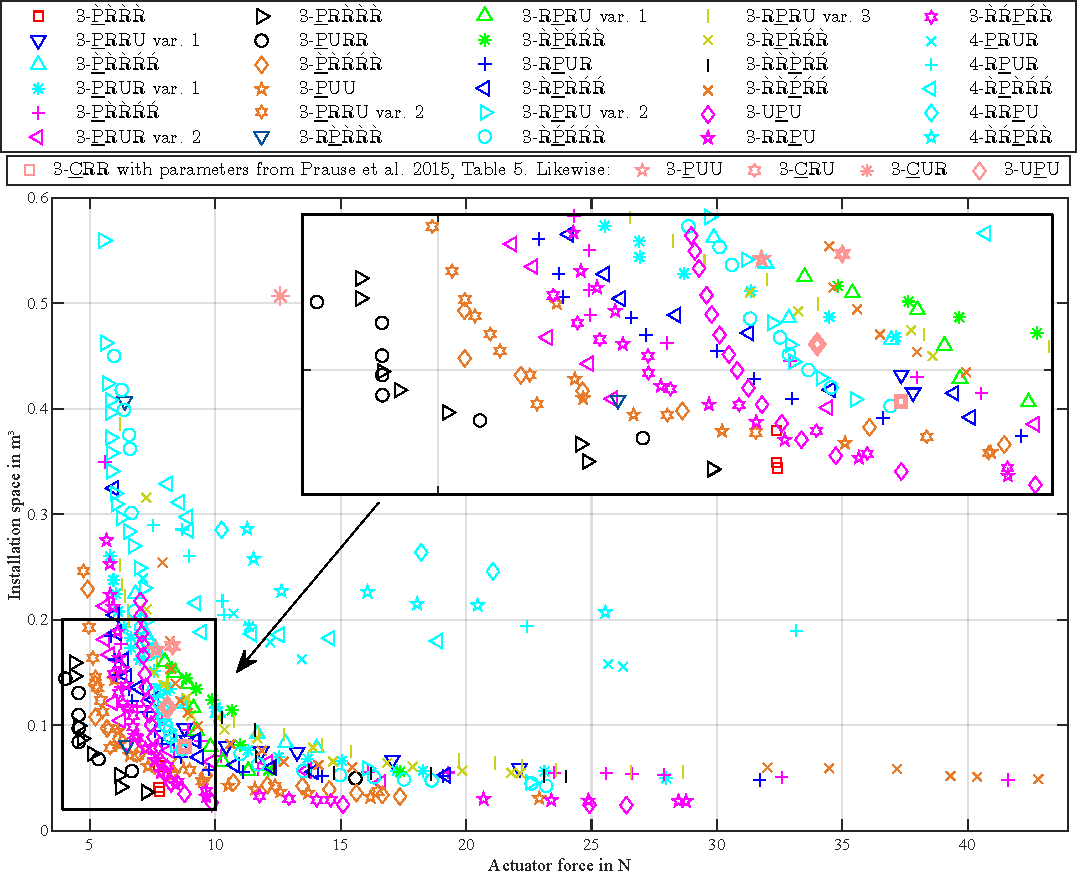
\includegraphics{Figures/handlingpkm_pareto_actforce_installspace_groups_onlypoints_prismatic.pdf}
  \end{adjustwidth}
  \caption[Handling task: \propername{Pareto} fronts for robots with prismatic actuation using only 27 reference points]{\propername{Pareto} fronts for robots with prismatic actuation using only 27 reference points.}%
\label{fig:handlingpkm_pareto_prismatic_onlypoints}
\end{figure}


\begin{figure}[H]
%
\begin{adjustwidth}{-\extralength}{0cm}
  \centering
  \graphicspath{{Figures}}
  \input{./Figures/handlingpkm_robots_reference.pdf_tex}
\end{adjustwidth}
%
\caption{\hl{Visualization} %
  %
  of the 3T0R parallel robots with parameters from \cite{PrauseChaCor2015}, listed in the bottom of Tables~\ref{tab:handlingpkm_results_pris}~and~\ref{tab:handlingpkm_results_pris_dh}.}
\label{fig:handlingpkm_robots_reference}
\end{figure}

\begin{figure}[H]
\vspace{0.1cm} %
\begin{adjustwidth}{-\extralength}{0cm}
  %
  \begin{overpic}
    {Figures/boxplots_handlingpkm/handlingpkm_boxplot_actforce_PrauseChaCor2015_collcheck1.pdf}
    \put(110,0){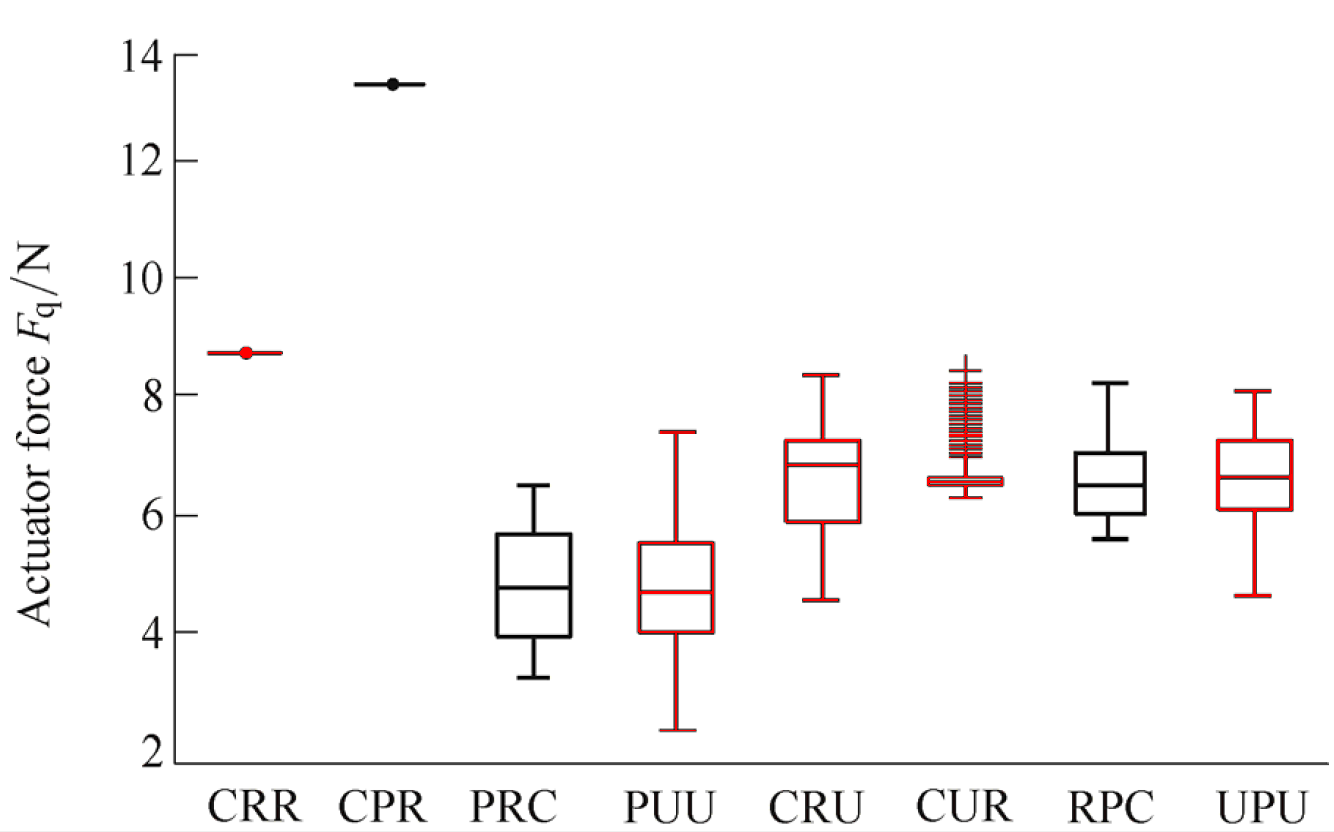
\includegraphics[width=8.2cm]{Figures/boxplots_handlingpkm/PrauseChaCor2015_Fig5.png}}
    \put(0,0){\textbf{(a)}}
    \put(110,0){\textbf{(b)}}
  \end{overpic} \\[0.5cm]
  \begin{overpic}
    {Figures/boxplots_handlingpkm/handlingpkm_boxplot_poserr_PrauseChaCor2015_collcheck1.pdf}
    \put(110,0){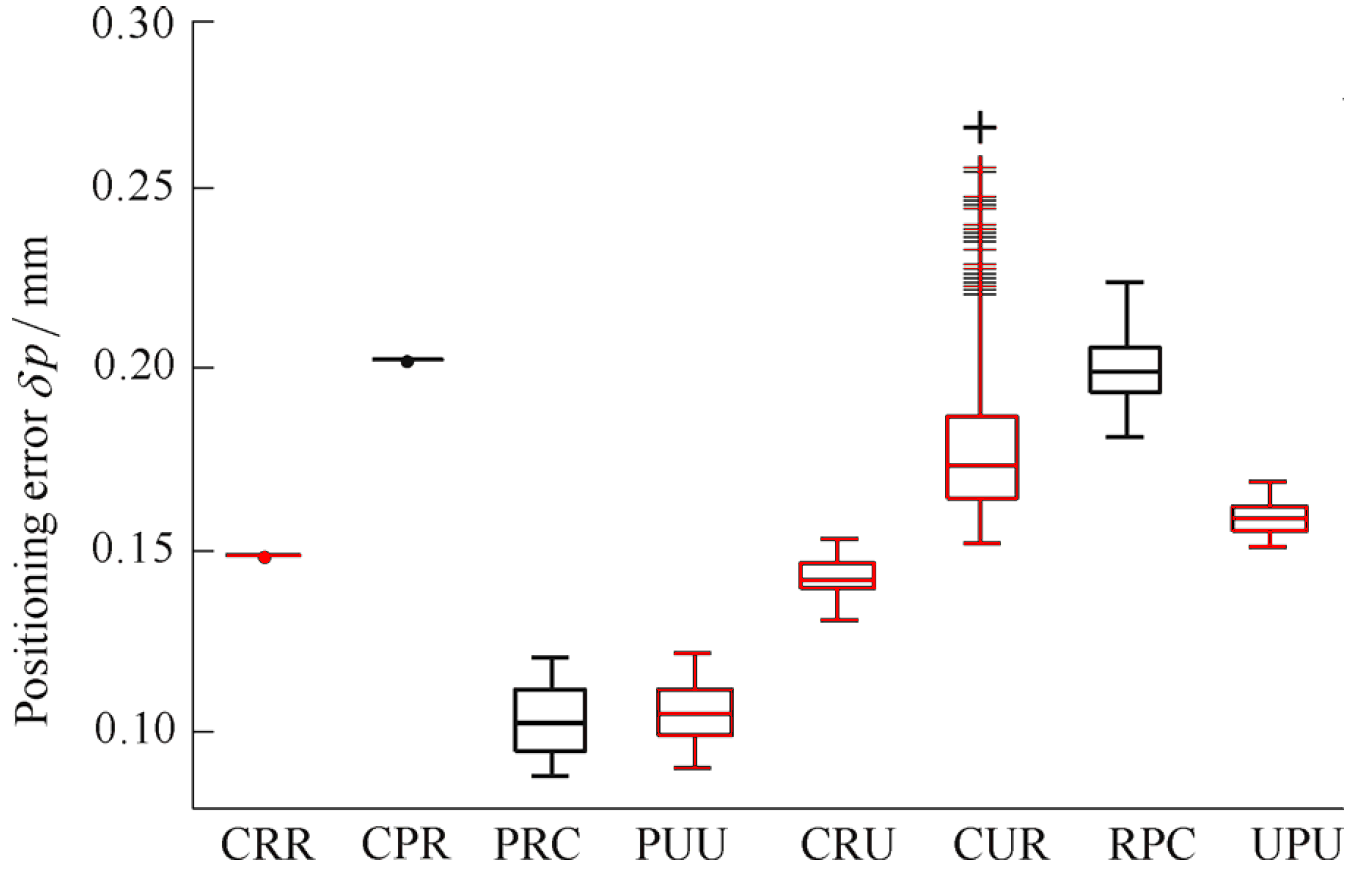
\includegraphics[height=4.9cm]{Figures/boxplots_handlingpkm/PrauseChaCor2015_Fig9.png}}
    \put(0,0){\textbf{(c)}}
    \put(110,0){\textbf{(d)}}
  \end{overpic} \\[0.5cm]
  \begin{overpic}
    {Figures/boxplots_handlingpkm/handlingpkm_boxplot_dexterity_PrauseChaCor2015_collcheck1.pdf}
    \put(110,0){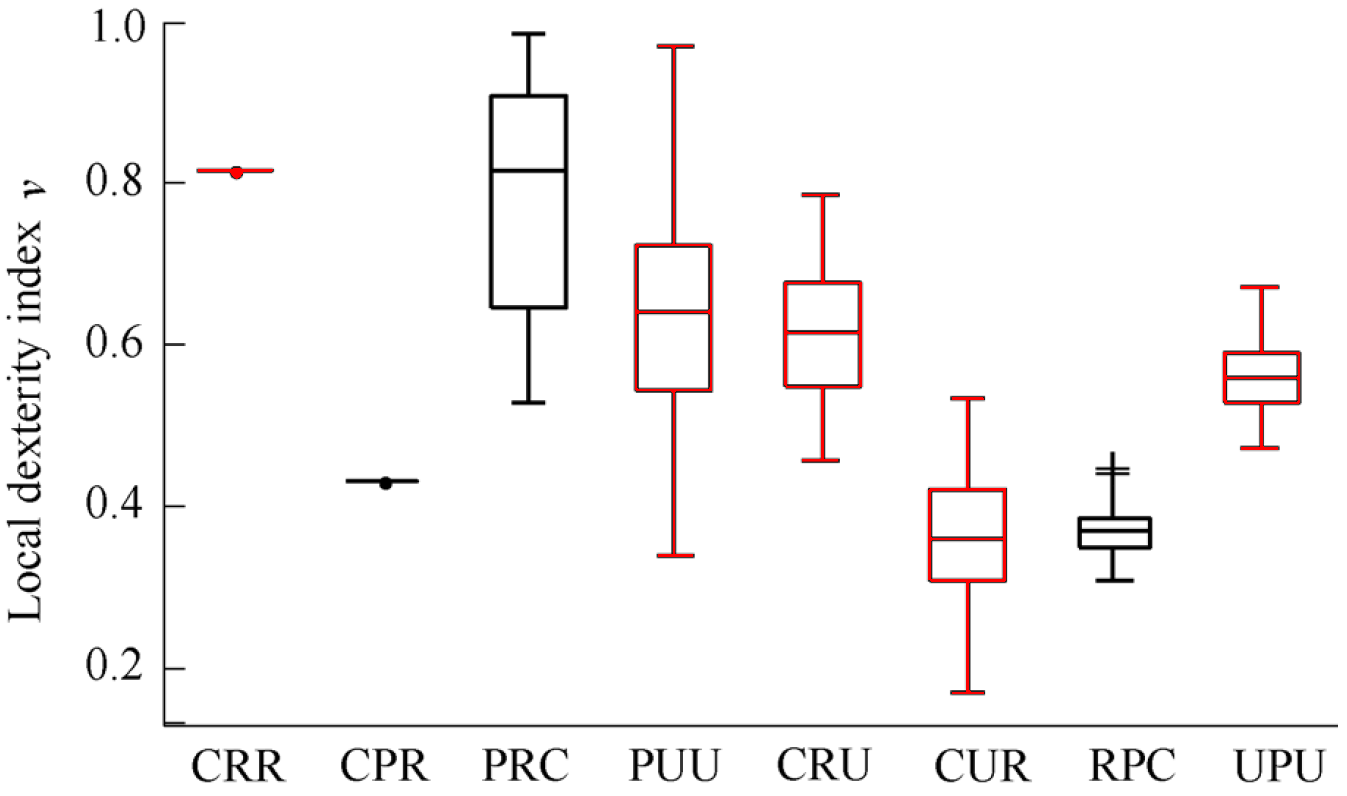
\includegraphics[height=4.9cm]{Figures/boxplots_handlingpkm/PrauseChaCor2015_Fig10.png}}
    \put(0,0){\textbf{(e)}}
    \put(110,0){\textbf{(f)}}
  \end{overpic} \\[0.15cm]
\end{adjustwidth}
%
\caption{Distribution of actuator force (\textbf{a},\textbf{b}), position error/precision (\textbf{c},\textbf{d}), and dexterity (\textbf{e},\textbf{f}) as performance criterion computed with parameters from Table~4 of \cite{PrauseChaCor2015} with this paper's implementation (left side) in comparison to the {original} results obtained from \cite{PrauseChaCor2015} (right side, with structures for comparison in red)}
\label{fig:handlingpkm_boxplot_PrauseChaCor2015}
%
\end{figure}

%

%
%
%
%
%
%
%
%
%

%


\begin{figure}[H]
\begin{adjustwidth}{-\extralength}{0cm}
  \centering
  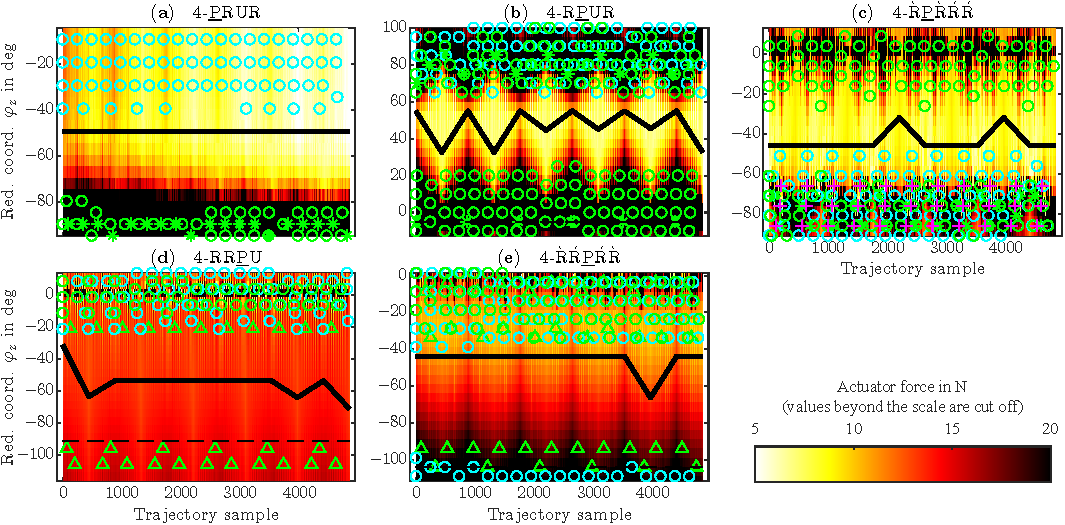
\includegraphics{Figures/handlingpkm_perfmaps_default_prismatic_multi_actforce_maxactforce.pdf}
\end{adjustwidth}
\caption{Performance
  maps for the prismatic-actuation parallel robots of Figure~\ref{fig:handlingpkm_robots_3T1R_pris} with maximum actuator force as IK objective and heat-map criterion. For marker legend, see below in Figure~\ref{fig:handlingpkm_perfmaps_multi_actforce_rev}.}
\label{fig:handlingpkm_perfmaps_multi_actforce_pris}
\end{figure}

\vspace{-12pt}
\begin{figure}[H]
\begin{adjustwidth}{-\extralength}{0cm}
  \centering
  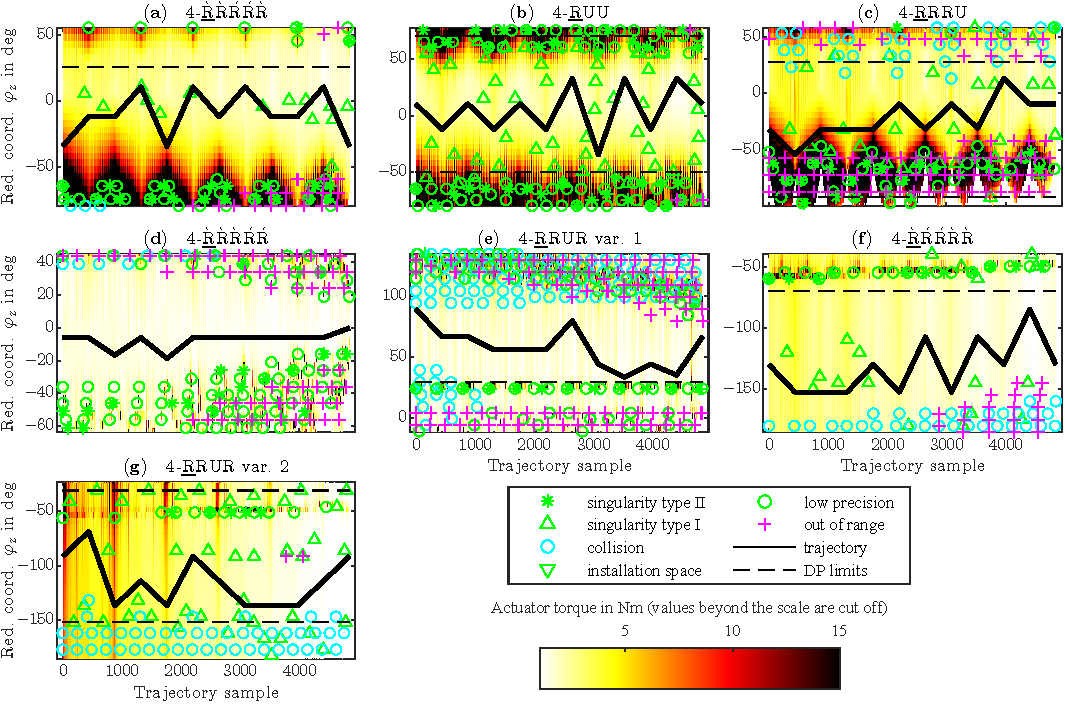
\includegraphics{Figures/handlingpkm_perfmaps_default_revolute_multi_actforce_maxactforce.pdf}
\end{adjustwidth}
\caption{Performance
  maps for the  revolute-actuation parallel robots of Figure~\ref{fig:handlingpkm_robots_3T1R_rev} with maximum actuator torque as IK objective and heat-map criterion.}
\label{fig:handlingpkm_perfmaps_multi_actforce_rev}
\end{figure}

\begin{figure}[H]
\begin{adjustwidth}{-\extralength}{0cm}
  \centering
  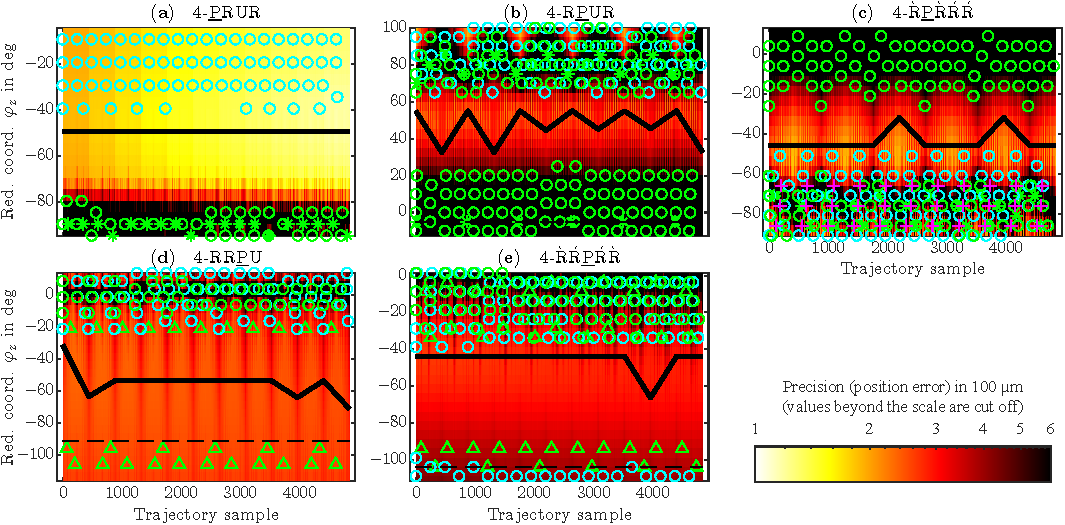
\includegraphics{Figures/handlingpkm_perfmaps_default_prismatic_multi_positionerror_maxactforce.pdf}
\end{adjustwidth}
\caption{Performance
  maps for the prismatic-actuation parallel robots of Figure~\ref{fig:handlingpkm_robots_3T1R_pris} with position error (precision) as heat-map criterion and trajectory from Figure~\ref{fig:handlingpkm_perfmaps_multi_actforce_pris}. For marker legend, see below in Figure~\ref{fig:handlingpkm_perfmaps_multi_poserr_rev}.}
\label{fig:handlingpkm_perfmaps_multi_poserr_pris}
\end{figure}

\vspace{-12pt}
\begin{figure}[H]
\begin{adjustwidth}{-\extralength}{0cm}
  \centering
  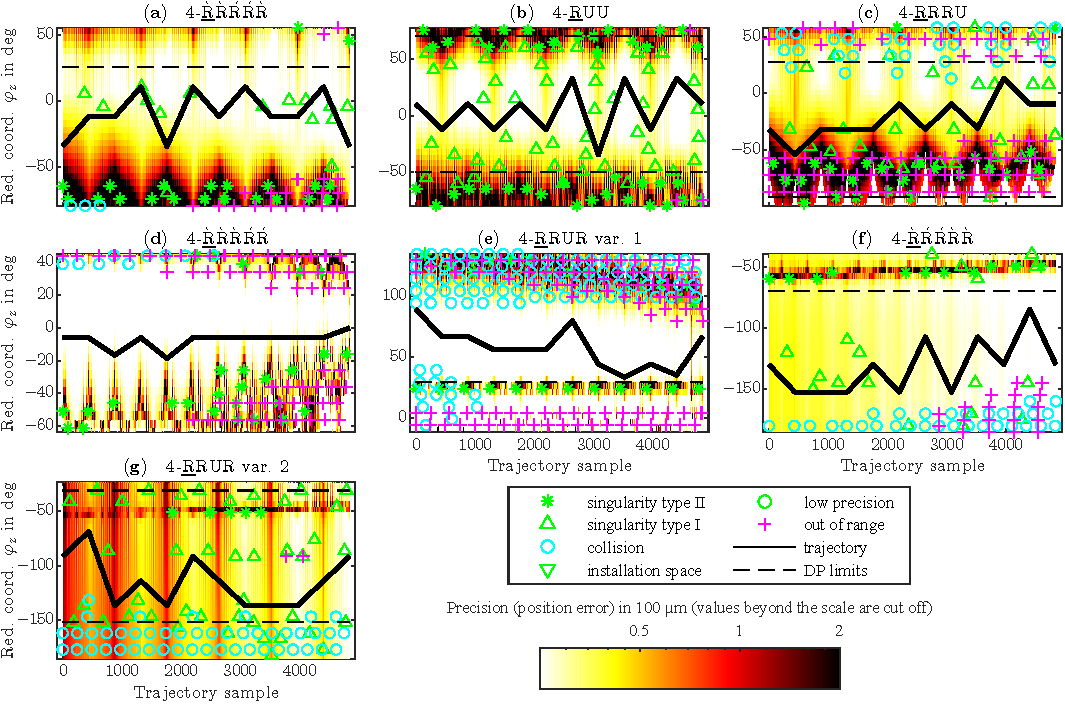
\includegraphics{Figures/handlingpkm_perfmaps_default_revolute_multi_positionerror_maxactforce.pdf}
\end{adjustwidth}
\caption{Performance
  maps for the revolute-actuation parallel robots of Figure~\ref{fig:handlingpkm_robots_3T1R_rev} with position error as heat-map criterion and trajectory from Figure~\ref{fig:handlingpkm_perfmaps_multi_actforce_rev}. Color scale is different than in Figure~\ref{fig:handlingpkm_perfmaps_multi_poserr_pris}~above.}
\label{fig:handlingpkm_perfmaps_multi_poserr_rev}
\end{figure} 

\begin{figure}[H]
\begin{adjustwidth}{-\extralength}{0cm}
  \centering
  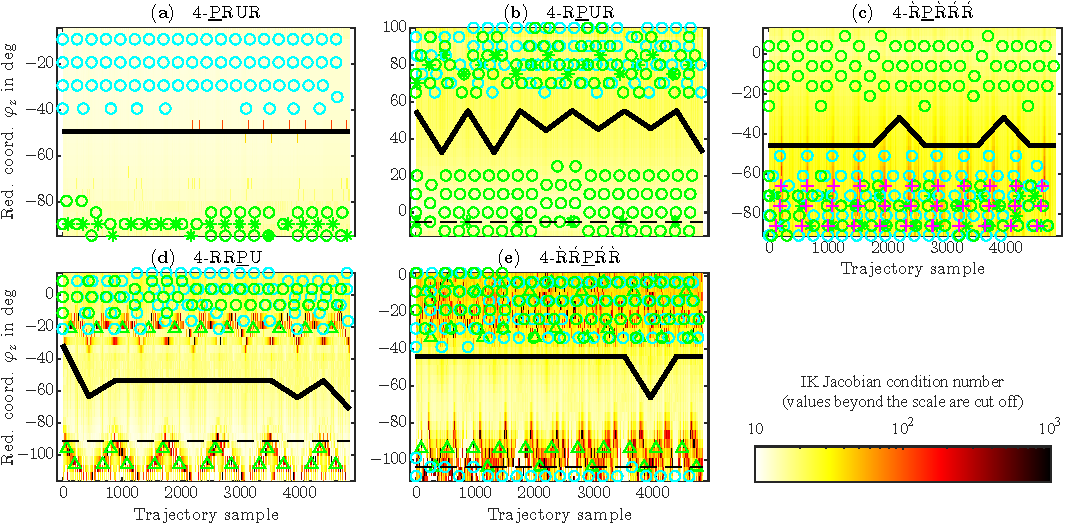
\includegraphics{Figures/handlingpkm_perfmaps_default_prismatic_multi_cond_ikjac_maxactforce.pdf}
\end{adjustwidth}
\caption{Performance
  maps for the prismatic-actuation parallel robots of Figure~\ref{fig:handlingpkm_robots_3T1R_pris} with IK-\propername{Jacobian} condition number as heat-map criterion and trajectory from Figure~\ref{fig:handlingpkm_perfmaps_multi_actforce_pris}. For marker legend, see below in Figure~\ref{fig:handlingpkm_perfmaps_multi_condikjac_rev}.}
\label{fig:handlingpkm_perfmaps_multi_condikjac_pris}
\end{figure} 

\vspace{-12pt}
\begin{figure}[H]
\begin{adjustwidth}{-\extralength}{0cm}
  \centering
  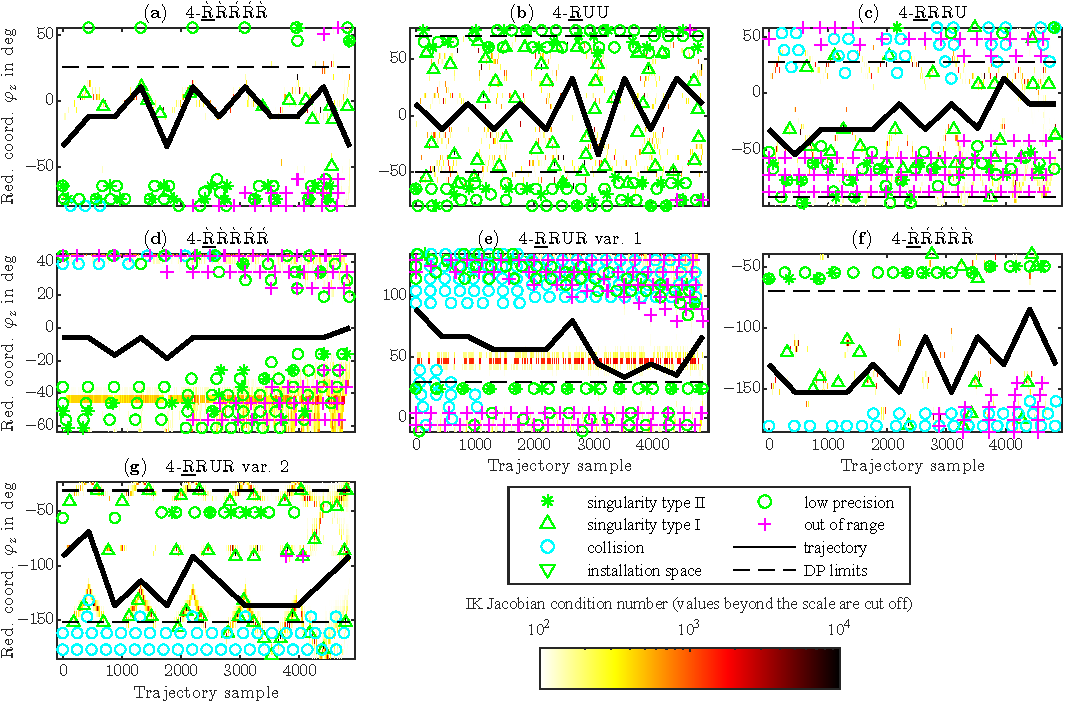
\includegraphics{Figures/handlingpkm_perfmaps_default_revolute_multi_cond_ikjac_maxactforce.pdf}
\end{adjustwidth}
\caption{Performance
  maps for the revolute-actuation parallel robots of Figure~\ref{fig:handlingpkm_robots_3T1R_rev} with IK-\propername{Jacobian} condition number as heat-map criterion and trajectory from Figure~\ref{fig:handlingpkm_perfmaps_multi_actforce_rev}. Color scale is different than in Figure~\ref{fig:handlingpkm_perfmaps_multi_condikjac_pris} above.}
\label{fig:handlingpkm_perfmaps_multi_condikjac_rev}
\end{figure} 
